\chapter{Neural networks as an approximation for the bridge function}
\label{Cap4}

%----------------------------------------------------------------------------------------
%	SECTION 1
%----------------------------------------------------------------------------------------

Neural networks can be used as \emph{universal approximators}~\cite{hornikMultilayerFeedforwardNetworks1989, hornikApproximationCapabilitiesMultilayer1991, cybenkoApproximationSuperpositionsSigmoidal1989},
i.e., they can take the form of any continuous function if and only if the conditions of the
\emph{universal approximation theorem} hold~\cite{parkMinimumWidthUniversal2020,zhouUniversalityDeepConvolutional2020}.
The aim of this chapter is to explore the hypothesis that a neural network might be 
useful as a bridge function parametrization in the closure expression for the 
Ornstein-Zernike equation~\cite{hansenTheorySimpleLiquids2013}.
If this is true, then choosing a particular approximation can be avoided for a given 
interaction potential, and leave the choice of the bridge function to the neural network 
itself, while simultaneously solving for the Ornstein-Zernike equation. It is intended to
explore the implications of two inquiries:

\begin{enumerate}[(a)]
    \item Is it possible to solve the Ornstein-Zernike equation using a neural network?
    \item If it is indeed possible, how good is the quality of the approximation for the pseudo hard sphere potential~\cite{baezUsingSecondVirial2018}?
\end{enumerate}

In this chapter, we show in detail the methodology created to answer these questions, and
the mathematical structure with which a neural network can be used to solve the
Ornstein-Zernike equation.
The results obtained are compared to those from Monte Carlo computer simulations to assess 
the quality of the solution.
In the appendices (\autoref{AppendixA}, \autoref{AppendixB}), the numerical algorithm used 
to solve the Ornstein-Zernike equation
is presented, along with a detailed computation of the gradients used for the
training scheme. Here, we shall focus only on the main results and the algorithm structure
in general.

\section{Parametrization of the bridge function}

The Ornstein-Zernike formalism is given by the following coupled equations~\cite{hansenTheorySimpleLiquids2013}
\begin{equation}
    \begin{aligned}
         & h(\vecr) = c(\vecr) +
        n \int_{V}
        c(\vecr^{\prime})
        h(\lvert \vecr - \vecr^{\prime} \rvert)
        d\vecr^{\prime} \\
         & c(\vecr)
        = \exp{\left[
                -  \beta u(\vecr)
                +  \gamma(\vecr)
                + B(\vecr)
                \right]} -
        \gamma(\vecr)
        - 1 ,
    \end{aligned}
    \label{eq:oz1}
\end{equation}
with the already known notation for each quantity (\textcolor{red}{Ref a marco teórico}).

Let $\nnet$ be a neural network with weights $\theta$. The main hypothesis
of this chapter is that $\nnet$ can replace the bridge function $B(\vecr)$
in the previous equation, which will yield the following expression for
the closure relation

\begin{equation}
    c(\vecr) = \exp{\left[
            -  \beta u(\vecr)
            +  \gamma(\vecr)
            + \nnet
            \right]} -
    \gamma(\vecr)
    - 1 .
    \label{eq:parametrizacion}
\end{equation}

With this new expression, the main problem to solve is to find the weights
of $\nnet$ that can successfully solve the Ornstein-Zernike equation
for a given interaction potential, $\beta u(\vecr)$.

%----------------------------------------------------------------------------------------
%	SECTION 2
%----------------------------------------------------------------------------------------

\section{Training scheme}
Now that a parametrization is defined, a way to fit the weights of the neural network must
be devised. This new numerical scheme must also be able to solve the OZ equation, while
simultaneously finding the appropiate weights for $\nnet$.

\subsection{Cost function}
It was mentioned previously that the main problem is to find the weights of
$\nnet$ that can successfully solve the Ornstein-Zernike equation
for a given interaction potential.
To solve such a problem, a \textbf{cost function} must be defined, and be used as part of
a \emph{minimization} problem.

To define such a function, we consider the successive approximations obtained from the
iterative Piccard scheme to solve the OZ equation, $\left\{\gamma_1(\vecr), \gamma_2(\vecr), \dots, \gamma_n(\vecr)\right\}$.
From this, we expect to have found a solution when each approximation
is \emph{close enough} to the previous one. This can be translated into the following
cost function
\begin{equation}
    J(\theta) = \left[\gamma_{n}(\vecr, \theta) - \gamma_{n-1}(\vecr, \theta) \right]^2 ,
    \label{eq:costo}
\end{equation}
where $\gamma_{n}(\vecr, \theta)$ is the $n$-th approximation of the indirect
correlation function, $\gamma(\vecr)$.
The notation $\gamma(\vecr, \theta)$ indicates that the function now depends
on the weights of the neural network, as seen in \autoref{eq:parametrizacion}.
This means that, if the weights of $\nnet$ change, we should expect a change in the output
from the $\gamma$ function.

Another way of looking at \autoref{eq:costo} is that we require that the last 
two approximations of the $\gamma$ function in each iteration from the numerical scheme to 
be equal within a tolerance value, or upper bound. This will enforce a change on the 
weights every time both approximations deviate between them.

\subsection{Optimization problem}
With a cost function at hand, an optimization problem can be defined such that the
weights of $\nnet$ will be adjusted properly.

This optimization problem is in fact an \emph{unconstrained optimization problem},
and it is defined simply as

\begin{equation}
    \begin{aligned}
         & \underset{\theta \in \mathbb{R}^n}{\text{min}}
         & & J(\theta) .
    \end{aligned}
    \label{eq:optimizacion}
\end{equation}

This formulation is just a search for the best values of the weights that minimize
the squared difference between successive approximations. We denote these optimal values
as the \emph{minimizer}, or $\theta^{*}$, such that $J(\theta^{*})$ is a minimum.
This optimization problem can be solved iteratively, along with the solution of the
OZ equation, whose procedure to get a solution is also through an iterative process.

\subsection{Weight updates}
The iterative method employed to adjust the weights of $\nnet$ is based on the
\emph{gradient descent} method~\cite{nocedalNumericalOptimization2006}.
The most general update rule for a method based on gradient descent reads~\cite{goodfellowDeepLearning2016}
\begin{equation}
    \theta_{n+1} = \theta_n - \eta \nabla_{\theta} J(\theta) ,
    \label{eq:gradiente}
\end{equation}
where $\eta$ is known as the \emph{learning rate}, and it is a hyperparameter
that controls the step size at each iteration while moving toward the minimum
of a cost function. This value needs to be \emph{tuned} accordingly, so
that the method converges properly. By tuning the parameter we mean that this value
should change until the numerical scheme is stable enough, or provides the best
possible answer to the optimization problem.

Regardless the particular expression for the weight updates, every method
based on the gradient descent method \emph{requires} the gradient information from
the cost function with respect to the weights, $\nabla_{\theta} J(\theta)$.
In this particular case, the detailed computation of the gradient is described in
the \autoref{AppendixA}.
Once this information is obtained, all that is left is to build an algorithm that
can correctly use this training scheme and solve the OZ equation.

\subsection{Solving the Ornstein-Zernike equation with neural networks}
\label{subsec:oz-solution}

Having described all the necessary elements needed, a general layout for the solution
of the Ornstein-Zernike using neural networks is now presented.

Thus, we propose the following steps to solve the OZ equation using the parametrization
described by \autoref{eq:parametrizacion}:

\begin{enumerate}
    \item Given a particular interaction potential $\beta u(\vecr)$, \autoref{eq:parametrizacion} is used to obtain the value of the direct correlation function $c(\vecr)$. In this step, an initial value for $\gamma_{n}(\vecr)$ is needed, which is initialized based on the five-point Ng methodology shown in \autoref{AppendixB}. The weights of the neural network $\nnet$ are initialized randomly. The initialization method is discussed in detail in the next section.
    \item The newly found function $c(\vecr)$ is transformed to a reciprocal space by means of the Fourier transform yielding the new function $\hat{c}(\veck)$.
    \item Then, the full OZ equation(\textcolor{red}{Ref a ec marco teórico}) is Fourier transformed. Using the information from the previous step, a new estimation of the indirect correlation function is obtained, $\hat{\gamma}_{n+1}(\veck, \theta)$.
    \item The Fourier transform is applied once again to return all the functions to real space. With this operation, a new estimation $\gamma_{n+1}(\vecr, \theta)$ is computed from the transformed function, $\hat{\gamma}_{n+1}(\veck, \theta)$.
    \item Both estimations, $\gamma_{n}$ and $\gamma_{n+1}$, are used to evaluate \autoref{eq:costo}. In this step, the gradient $\nabla_{\theta} J(\theta)$ is computed as well.
    \item The weights $\theta$ are updated using a gradient descent rule, similar to \autoref{eq:gradiente}, and the process is repeated from step 1. In the next iteration, the initial value for the indirect correlation function will be $\gamma_{n+1}$, and a new estimation $\gamma_{n+2}$ will be obtained. This process is repeated until convergence.
\end{enumerate}

\subsection{Convergence criterion}
The procedure described in the previous section is repeated indefinetely until convergence
is achieved. This convergence criterion is defined as follows

\begin{equation}
    \sum_{i=1}^{N} {\left( \gamma^{n+1}_{i} - \gamma^{n}_{i} \right)}^2 \leq \epsilon .
    \label{eq:tolerancia}
\end{equation}

This expression is also known as the \emph{mean squared error}~\cite{goodfellowDeepLearning2016}.
Here, we sum all the $N$ elements of the squared difference between estimates $\gamma_{n+1}$
and $\gamma_{n}$. The paramater $\epsilon$ is a tolerance value that indicates an 
upper bound for the error between estimations. When the computed error is below this 
tolerance value, we consider the algorithm to \emph{have converged to a particular minimum}.
This means that the weights are adjusted until the successive estimations of the $\gamma$
functions are equal between them, up to the defined tolerance $\epsilon$.
Specifically, the numerical tolerance in all the experiments was fixed to be
$\epsilon = \num{1e-5}$ to allow for a robust exploration of the search space, without being
too restrictive. When using a lower value of $\epsilon,$ it was observed that the results 
were not improving at all (data not shown).

%----------------------------------------------------------------------------------------
%	SECTION 3
%----------------------------------------------------------------------------------------
\section{Implementation}
In this section we detail the most important aspects about the implementation of the
method described in the previous section. This includes the topology of the neural network,
the optimization method, and the choice of activation function. The physical parameters
as well as the computer simulations methods used to solve the OZ equation are also outlined.

\subsection{Choice of optimization algorithm}
The general rule for the weight update based on \autoref{eq:gradiente} was
implemented to solve the optimization problem, but numerical inconsistencies rendered this 
method unstable and convergence was almost never achieved.

To solve this issue, the \emph{Adam}~\cite{kingmaAdamMethodStochastic2017} optimization 
method was chosen. This optimization method is an excellent choice for the training
of neural networks, even more when the gradient is expected to be \emph{sparse}, i.e.
most of the elements of the gradient itself are zeros.
The \emph{Adam} method uses several rules to adjust the descent direction of the gradient,
as well as the hyperparameters related to the acceleration mechanism of the method.
Notably, there are two important hyperparameters used in the method; $\beta_1$,
which controls the moving average of the computed gradient; and $\beta_2$, which controls
the value of the gradient squared~\cite{kingmaAdamMethodStochastic2017}. Both parameters 
are necessary for the optimal convergence of the algorithm.

The equations that define the optimization method are the following
\begin{equation}
    \begin{aligned}
        m_{t} &= \beta_1 m_{t-1} - (1 - \beta_1) \nabla_{\theta_{t-1}} J(\theta_{t-1}) \\
        s_{t} &= \beta_2 s_{t-1} + (1 - \beta_2) \nabla_{\theta_{t-1}} J(\theta_{t-1}) \odot \nabla_{\theta_{t-1}} J(\theta_{t-1}) \\
        \hat{m}_{t} &= \frac{m_{t}}{1 - \beta_1^t} \\
        \hat{s}_{t} &= \frac{s_{t}}{1 - \beta_2^t} \\
        \theta_{t} &= \theta_{t-1} + \eta \hat{m}_{t} \oslash \sqrt{\hat{s}_{t} + \varepsilon}
    \end{aligned}
    \label{eq:adam}
\end{equation}
where $\odot$ is the elementwise multiplication, or Hadamard product;
$\oslash$
is the elementwise division, or Hadamard division;
and $\varepsilon$ is a smoothing value to prevent division by zero~\cite{hornMatrixAnalysis2012}.
The index $t$ represents each of the updates, or iterations, done by the algorithm.

In the results presented in this chapter, the parameters were fixed to the ones reported
as optimal in the original work of the \emph{Adam}
method~\cite{kingmaAdamMethodStochastic2017}, which are
$\beta_1=\num{0.9}$ and $\beta_2=\num{0.999}$. It is important to note that this method
has its own mechanisms to control and modify the gradients, as well as the hyperparameters.
This makes it a \emph{hands-off} method, without the need to tune the hyperparameters.
The \emph{learning rate}, $\eta$ in \autoref{eq:gradiente}, was fixed to
$\eta=\num{1e-4}$ for all the experiments because when a larger value was used the 
optimization method did not converge properly, and the results were not useful to be 
presented here. In a more practical situation, the best
way to choose the value of $\eta$ is to employ \emph{grid search} and look for the value
that minimizes the error the most~\cite{hastieElementsStatisticalLearning2009}.

\subsection{Neural network topology}

\begin{figure}[t]
    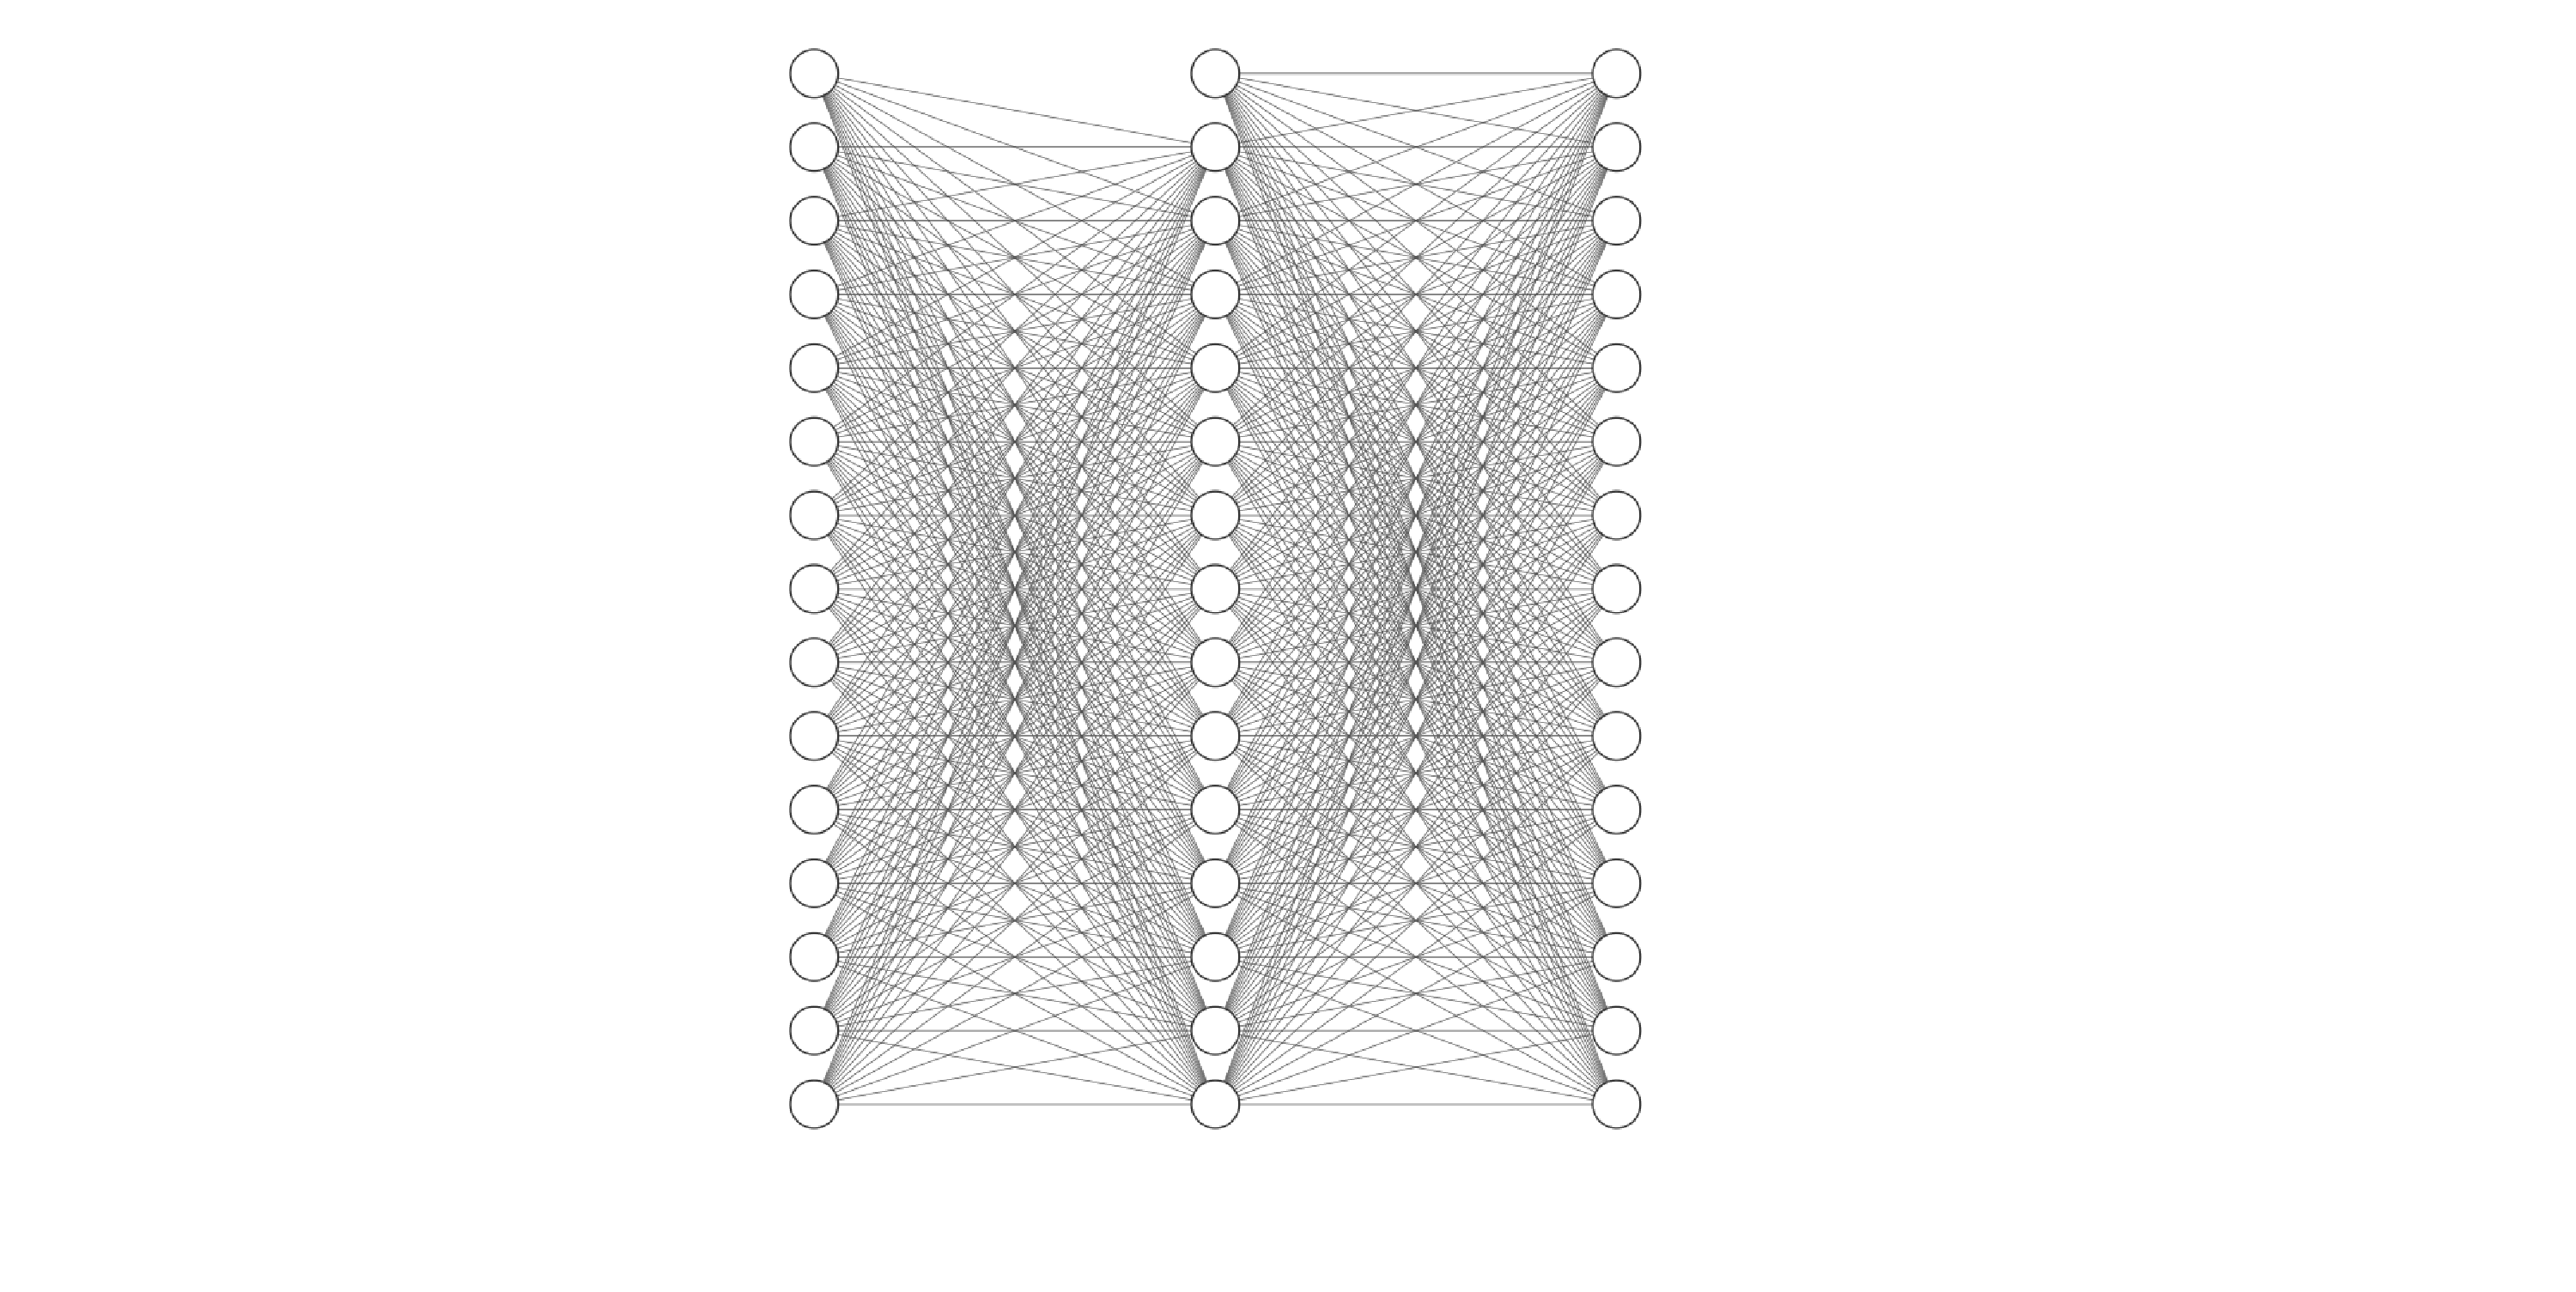
\includegraphics[width=\textwidth]{figuras/capitulo-4/neural-network.pdf}
    \vspace{-1.5cm}
    \caption[General schematics of a neural network.]{Cartoon of a fully connected multilayer neural network. Note that there is one \emph{hidden layer}. The circles represent the \emph{nodes} or \emph{units} used to compute the final output. These nodes are being evaluated by an activation function to account for nonlinearities. The top-most nodes that seem different from the main nodes are known as the \emph{bias} nodes. The real topology used in this chapter is larger, with many more nodes and connections, but the topology is the same.}
    \label{fig:nn-esquema}
\end{figure}

The neural network topology used in all the experiments is identical to the one
shown in \autoref{fig:nn-esquema}, with the exception of the number of nodes in each layer.
In particular, the neural network is made of \emph{three layers} fully connected between 
them.
There is an \emph{input} layer, one \emph{hidden} layer, and a final \emph{output} layer.
All layers have the same number of nodes, which is 4096. Additional nodes are added to the
final two layers that serve as the \emph{bias} terms.

All the weights must be initialized appropiately, and in this case the Glorot uniform
distribution was used~\cite{glorotUnderstandingDifficultyTraining2010}, which has proven
to be an excellent way to help the convergence of neural networks.
When using the Glorot uniform distribution, the weights are initialized as
$
\theta_{ij} \sim \mathcal{U} \left[ -\frac{6}{\sqrt{(in + out)}},
\frac{6}{\sqrt{(in + out)}} \right]
$,
where $\mathcal{U}$ is the uniform probability distribution;
$in$ represents the number of units in the input layer; and $out$ the number of
units in the output layer. All bias nodes were initialized to be zero.

The activation function used was the \emph{ReLU}~\cite{glorotDeepSparseRectifier2011}
function, which has the form
\begin{equation*}
    \text{ReLU}(x) = \max{(0, x)} .
\end{equation*}

This activation function is applied to all the nodes in the layers, with the exception
of the input layer. This function was chosen due to the fact that the other most common
functions ($\tanh, \text{softmax}$, etc.) were numerically unstable in the training process 
of the neural network (data not shown).

\subsection{Physical parameters and simulations}

To solve the OZ equation a cutoff radius of $r_c=7\sigma$ was used, where $\sigma$ is the
particle diameter and it was fixed to be $\sigma=1$.
The interaction potential used was the pseudo hard sphere potential (\textcolor{red}{Ref a ec.}), both
for the solution of the OZ equation, as well as the results obtained from computer simulations.

Seven different densities were explored in the range $\phi \in [\num{0.15}, \num{0.45}]$, 
with $\Delta \phi = \num{0.05}$.
For each density value, a grid of 70 points was used to ensure convergence of the iterative
algorithm when solving for the OZ equation. This was not the case for the computer 
simulations, where such partition is not needed.

Computer simulations results were obtained using the traditional Monte Carlo simulation
method within the Metropolis scheme for the $NVT$ ensemble (\textcolor{red}{Ref a marco teórico}). In every experiment, the total number of particles was 2197,
the system was equilibrated for a total of 10 million Monte Carlo steps, and the radial
distribution functions were obtained from the sampling of 7 million Monte Carlo steps, after
the system was equilibrated. To reduce the number of computations, a cutoff radius of
half the size of the simulation box was used for the evaluation of the interaction 
potential. Periodic boundary conditions in all spatial dimensions were used accordingly. 
The same pseudo hard sphere potential (\textcolor{red}{Ref a ecuación}) was used, instead
of the true hard sphere potential, for a fair comparison with the results obtained from the 
OZ equation.

%----------------------------------------------------------------------------------------
%	SECTION 4
%----------------------------------------------------------------------------------------
\section{Results}
It is now time to investigate the results obtained from the proposed methodology, using all the elements previously described.
The main point of discussion will be the radial distribution
function \textemdash $g(r^*)$ \textemdash for different values of densities, both in the
low and high density regimes.

\subsection{Low densities}
In this section we will deal with the low 
density values ranging from $\phi=\numlist[list-pair-separator={\enspace\text{to}\enspace}]{0.15;0.25}$, which are shown in \autoref{fig:rdf15} and \autoref{fig:rdf25}, respectively.
The results show that, at low densities, the HNC and neural network approximations are
more precise than the modified Verlet approximation. Although at first glance, all
approximations seem to fall short compared to computer simulations. This is particularly 
noticeable in the neighborhood around the second peak, which is shown in the insets 
of \autoref{fig:rdf15} and \autoref{fig:rdf25}.
Additionally, it is important to note that the neural network approximation is slightly
more precise than the HNC approximation, which can be qualitatively appraised by observing 
the estimation of the main peak in the radial distribution function. This peak can be found 
in the vicinity of $r^* = 1$. Nevertheless, it is still overestimated, which is the 
same case for the HNC approximation. However, this is not the case for the modified Verlet 
approximation, which underestimates the main peak.

In like manner, the functional form of $g(r^*)$ is important to study closely.
For the HNC and neural network approximations, it appears to have the same form between 
both approximations, and it might as well be the same.
This would imply that, somehow, the weights of the neural network
were updated enough such that a minimum was found, and this minimum was very close to the
HNC approximation. In other words, the results suggest that the weights are very close to
zero, such that when the neural network is evaluated, the output is close to the
result obtained from the HNC approximation.
Another important aspect to observe is that this functional form is marginally different
to the one seen from computer simulations, and that the modified Verlet approximation is 
closer to the form found in the computer simulations results.

\subsection{High densities}
We now turn our attention to the high density values, namely,
$\phi=\numlist[list-pair-separator={\enspace\text{and}\enspace}]{0.35; 0.45}$,
represented in \autoref{fig:rdf35} and \ref{fig:rdf45}.
In the same spirit as before with the low densities, the HNC and neural network 
approximations are not precise when compared to computer simulations. In this case,
the modified Verlet bridge function approximation is even more precise, which was expected.
This is because the HNC approximation is a very good approximation for long range
interaction potentials (\textcolor{red}{Ref faltante}), whereas the modified Verlet is 
better suited for short range potentials, such as the one studied here.
In this case, modified Verlet is the most precise of the approximations used, which
can be inpsected in \autoref{fig:rdf35} and \autoref{fig:rdf45}, where the 
main peak is accurately estimated by the approximation when compared to Monte Carlo 
computer simulation results. However, both HNC and neural network approximations 
overestimate this quantity.

Further, the functional form of $g(r^*)$ computed with the neural network approximation 
is substantially different to the one obtained with computer simulations. Indeed, the result
obtained is similar to the one obtained with the HNC approximation, and both are imprecise 
approximations to the expected functional form; this was also the case for low densities.
This result is important, backing the hypothesis that the
neural network might reduce to the HNC approximation.
This would imply that the neural network is in fact approximating the bridge function
$B(\vecr) \approx 0$. If we now pay attention to the modified Verlet
approximation, again in \autoref{fig:rdf35} and \autoref{fig:rdf45}, 
we can see that the modified Verlet bridge function is the most precise
out of all the set of bridge functions used. In other words, we observe that this
estimation provides a precise prediction of the main peak, as can be seen when compared to 
the results obtained from computer simulations, which are almost identical.

\begin{figure}[t]
    \centering
    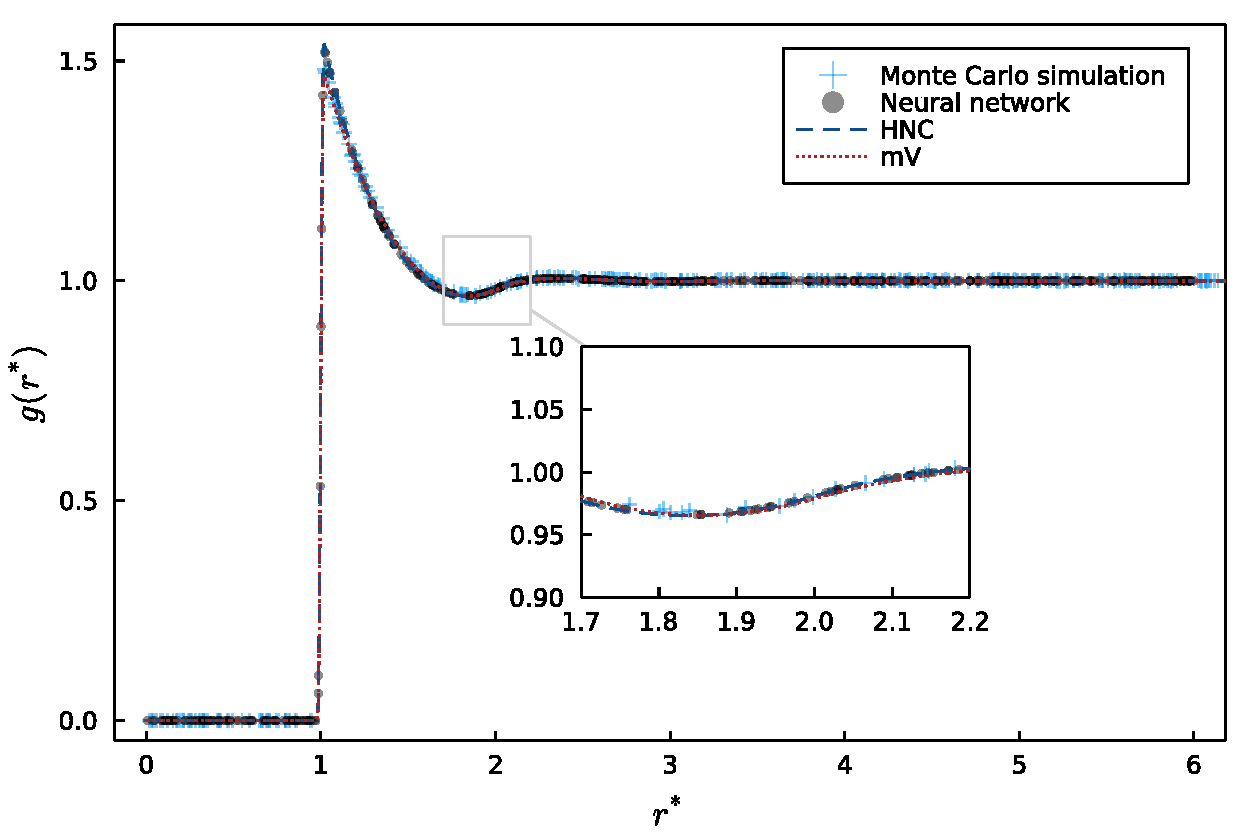
\includegraphics[width=\textwidth]{figuras/capitulo-4/comparison_p=0.15.pdf}
    \caption[Radial distribution function, $\phi=0.15$.]{Radial distribution function for $\phi=0.15$ obtained from Monte Carlo simulations, and three different approximations:
    \begin{enumerate*}[label=(\alph*),itemjoin={,\enspace}]
        \item \emph{mV}, (modified Verlet)
        \item \emph{HNC}, (Hypernetted Chain)
        \item \emph{NN}, (neural network approximation).
    \end{enumerate*}
    Inset shows the region close to the peak about $r^{*}=2$.
    }
    \label{fig:rdf15}
\end{figure}

\begin{figure}[t]
    \centering
    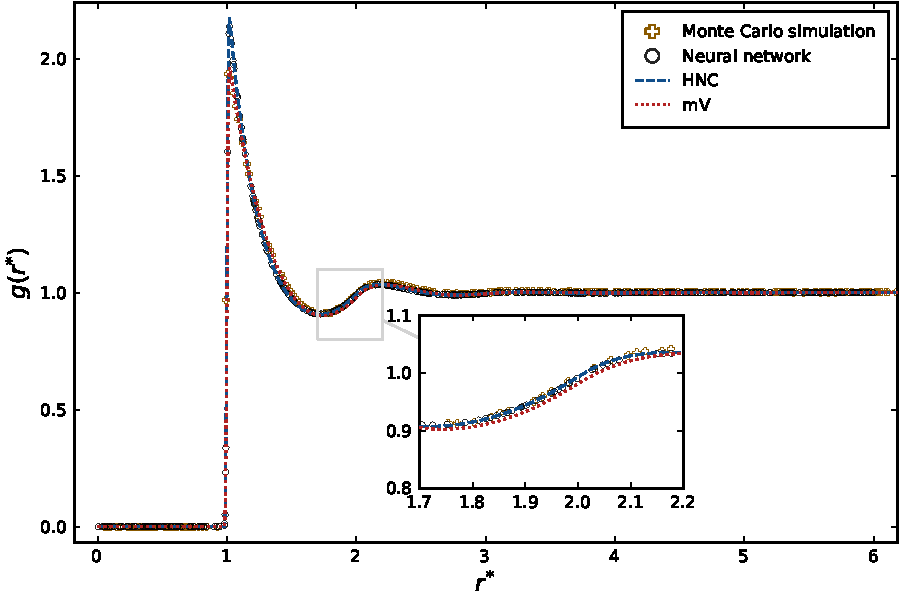
\includegraphics[width=\textwidth]{figuras/capitulo-4/comparison_p=0.25.pdf}
    \caption[Radial distribution function, $\phi=0.25$.]{Radial distribution function for $\phi=0.25$ obtained from Monte Carlo simulations, and three different approximations:
    \begin{enumerate*}[label=(\alph*),itemjoin={,\enspace}]
        \item \emph{mV}, (modified Verlet)
        \item \emph{HNC}, (Hypernetted Chain)
        \item \emph{NN}, (neural network approximation).
    \end{enumerate*}
    Inset shows the region close to the peak about $r^{*}=2$.
    }
    \label{fig:rdf25}
\end{figure}

\begin{figure}[t]
    \centering
    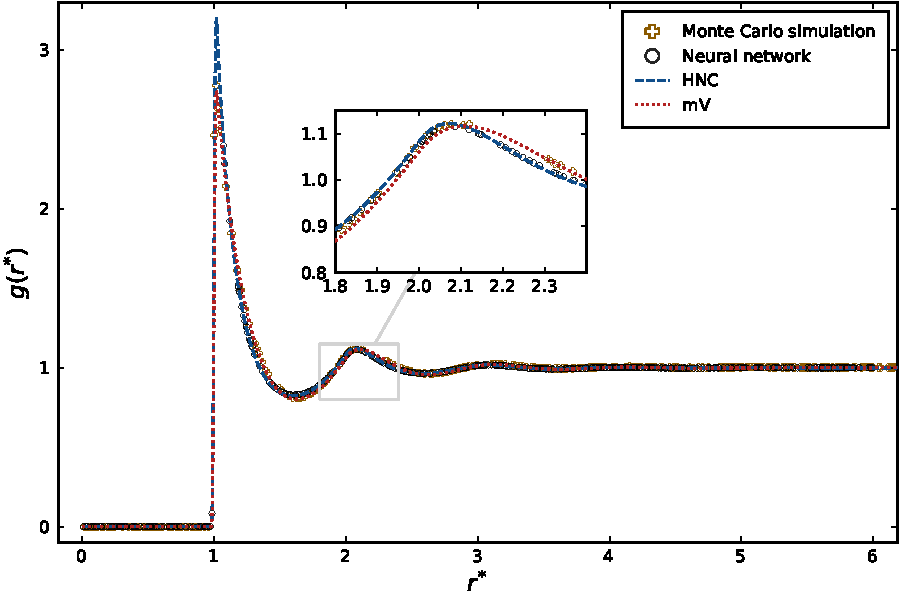
\includegraphics[width=\textwidth]{figuras/capitulo-4/comparison_p=0.35.pdf}
    \caption[Radial distribution function, $\phi=0.35$.]{Radial distribution function for $\phi=0.35$ obtained from Monte Carlo simulations, and three different approximations:
    \begin{enumerate*}[label=(\alph*),itemjoin={,\enspace}]
        \item \emph{mV}, (modified Verlet)
        \item \emph{HNC}, (Hypernetted Chain)
        \item \emph{NN}, (neural network approximation).
    \end{enumerate*}
    Inset shows the region close to the peak about $r^{*}=2$.
    }
    \label{fig:rdf35}
\end{figure}

\begin{figure}[t]
    \centering
    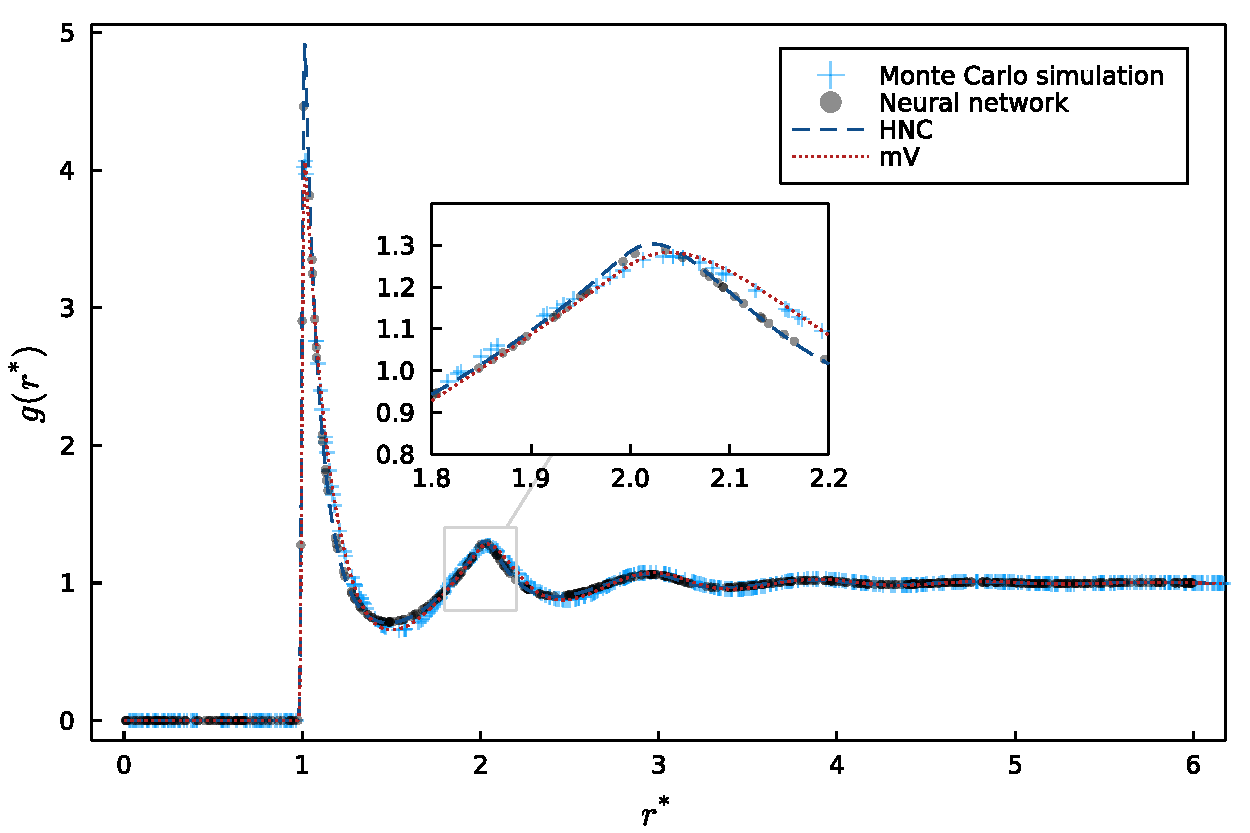
\includegraphics[width=\textwidth]{figuras/capitulo-4/comparison_p=0.45.pdf}
    \caption[Radial distribution function, $\phi=0.45$.]{Radial distribution function for $\phi=0.45$ obtained from Monte Carlo simulations, and three different approximations:
    \begin{enumerate*}[label=(\alph*),itemjoin={,\enspace}]
        \item \emph{mV}, (modified Verlet)
        \item \emph{HNC}, (Hypernetted Chain)
        \item \emph{NN}, (neural network approximation).
    \end{enumerate*}
    Inset shows the region close to the peak about $r^{*}=2$.
    }
    \label{fig:rdf45}
\end{figure}

\section{Discussion}
It would seem as though the neural network approximation reduces to the HNC
approximation, as seen in the results from the previous section. In this section
we shall investigate this matter in detail.
We will also continue the discussion of the results presented and try to make sense
of the training dynamics of the neural network. This is an important topic to
address due to the clear results that the neural network provides almost the same
result as the HNC approximation.

\subsection{Weight evolution of the neural network}

\begin{figure}[t]
    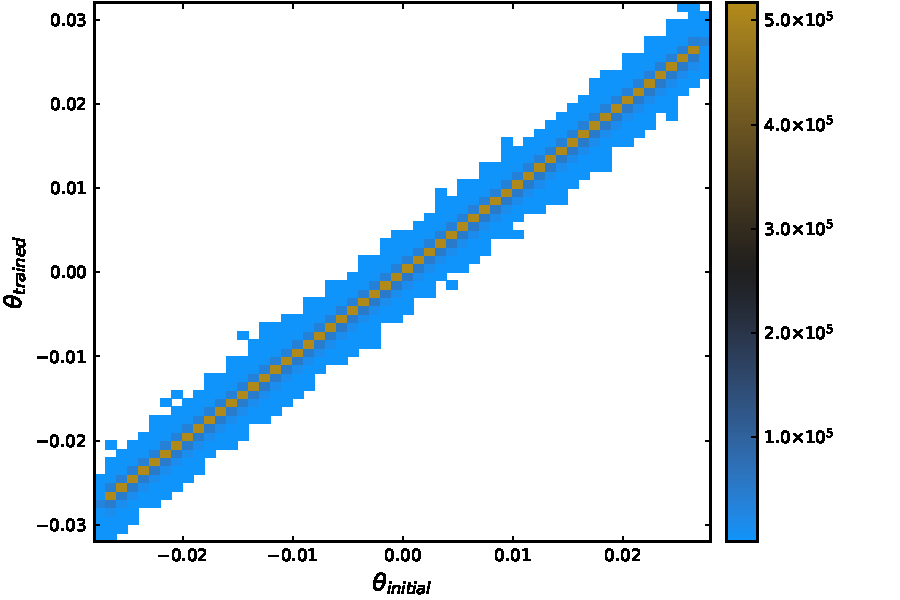
\includegraphics[width=\textwidth]{figuras/capitulo-4/weights_phi=0.15.pdf}
    \caption[Comparison between weights, $\phi=0.15$.]{Relation between the trained weights and the initial weights of $\nnet$ for $\phi=0.15$. The scale on the right-hand side represents the total number of instances for the trained-initial pair of weights.} 
    \label{fig:pesos15}
\end{figure}

We shall now examine the evolution of the weights $\theta$ from
$\nnet$, from the moment it was initialized to the moment its training finalized.
A histogram of this for the density values 
$\phi=\numlist[list-final-separator={\; \text{and} \;}]{0.15;0.25;0.35;0.45}$ 
can be seen in \autoref{fig:pesos15}, \autoref{fig:pesos25}, \autoref{fig:pesos35}, 
and \autoref{fig:pesos45}, respectively.
We can observe that the way the weights show a diagonal represent a linear relationship 
between the initial weights, $\theta_{i}$, and the trained weights, $\theta_{t}$. In other 
words, the weights follow the linear expression
$\theta_{t} = \alpha \theta_{i} + \beta + \epsilon$, with
$\epsilon \sim \mathcal{N}(\mu, \sigma^{2})$ a normal random variable with mean
$\mu$ and variance $\sigma^2$. The noise term can be any other continuous probability 
distribution, but without loss of generality the normal distribution was chosen for
our purposes. For now, we are not interested in the values of $\alpha$ or $\beta$,
but merely on the linear relationship between them.

One thing to notice is the fact that the higher the density value is, the larger
the variance turns out to be. If we observe the variance for the density
$\phi=0.15$ in \autoref{fig:pesos15}
we see that the variance is small due to the fact that the blue shaded region around
the diagonal is close to it. If we now see the same \autoref{fig:pesos45} for the 
density value of $\phi=0.45$ we observe that this shaded region is significantly larger.
This would mean that, at higher densities, the weights of $\nnet$ are more spread out
from the mean, and the neural network might have adjusted its weights to account for
different computations of the bridge function.

The most interesting part of this is the fact that the weights from initialization
do not change much throughout the training scheme, which would imply that a local minimum
has already been found. This might be the case, because HNC is actually a solution of
the OZ equation, and solutions around this particular approximation might as well be
solutions themselves.
This, however, does not answer the question of why the spread is larger when
higher densities are inspected.

\begin{figure}[t]
    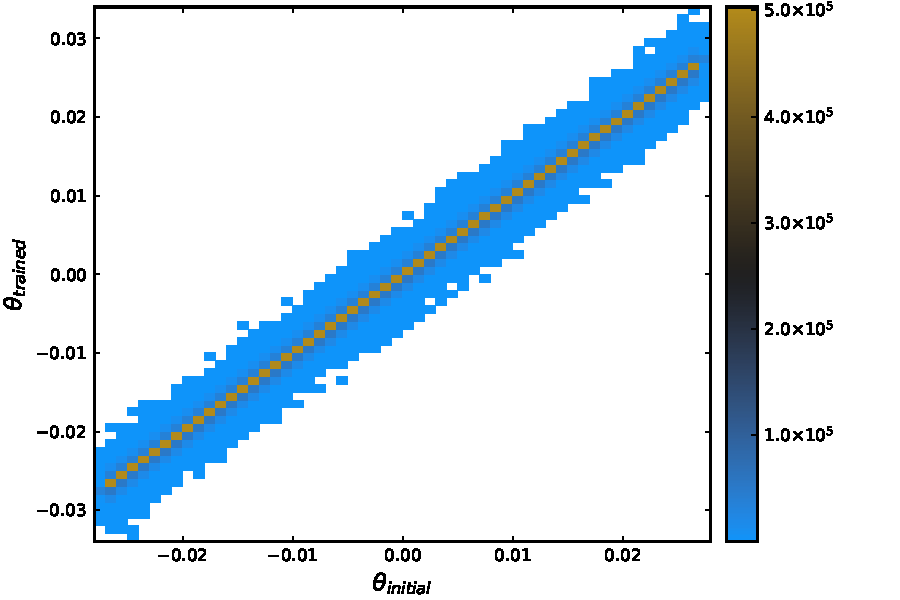
\includegraphics[width=\textwidth]{figuras/capitulo-4/weights_phi=0.25.pdf}
    \caption[Comparison between weights, $\phi=0.25$.]{Relation between the trained weights and the initial weights of $\nnet$ for $\phi=0.25$. The scale on the right-hand side represents the total number of instances for the trained-initial pair of weights.}
    \label{fig:pesos25}
\end{figure}

\subsection{The Hypernetted Chain approximation as a stable minimum}
It would seem that the way the weights are updated, albeit with minimal change from its
initial values, is due to the fact of already being near a minimum when the training starts.
We must recall that the weight update and neural network training is essentially an
optimization problem, and the main goal is to find a minimum
of the cost function in \autoref{eq:costo}. With the results presented so far, it might be
possible to postulate that the \emph{HNC approximation is a stable minimum} for the
neural network $\nnet$.
This would answer the question of why the weights of the neural network during training
explored in the previous section did not change very much throughout the numerical scheme.
Because if we have already found a minimum, the optimization algorithm might end up
oscillating in the proximity of this value.

On the other hand, this idea could also give answer to the question of why the spread
is larger for higher density values. If we pay close attention to the neural network bridge
approximation results for the \emph{low density} values in \autoref{fig:rdf15}, we can see 
that although all the bridge functions give a low accuracy estimation of the second peak as shown in the inset within the figure. However, for the main peak the neural network 
approximation is accurate.
If we now observe \autoref{fig:rdf45}, which refers to the \emph{high density} value,
we can see that the estimation is a poor one.

Let us now relate this to the weight evolution. For the \emph{low density} regime, the 
weight evolution has a \emph{lower variance}; for the \emph{high density} regime, a \emph{higher variance} is observed in the weight evolution.
This suggests that, for \emph{lower density} values, there was no need to adjust the
weights more than shown in \autoref{fig:pesos15} because the approximation is accurate
enough. However, for the \emph{higher density} values, the approximation is not good enough
and the optimization method was trying to adjust the weights accordingly, even if
unsuccessfully.
Thus, by oscillating near the value of zero, which represents the HNC bridge function,
the neural network does not need additional information and generates a bridge function 
approximation that reproduces the results from the HNC closure relation.

Having a stable minimum when training starts would mean that the neural network does not
learn enough, and will alway keep its weights tightly centered about the mean of this
minimum. Still, this implies that other minima are available for the neural network as long
as the weights are correctly initialized, or a probability distribution centered about
a particular minima is used.

\begin{figure}[t]
    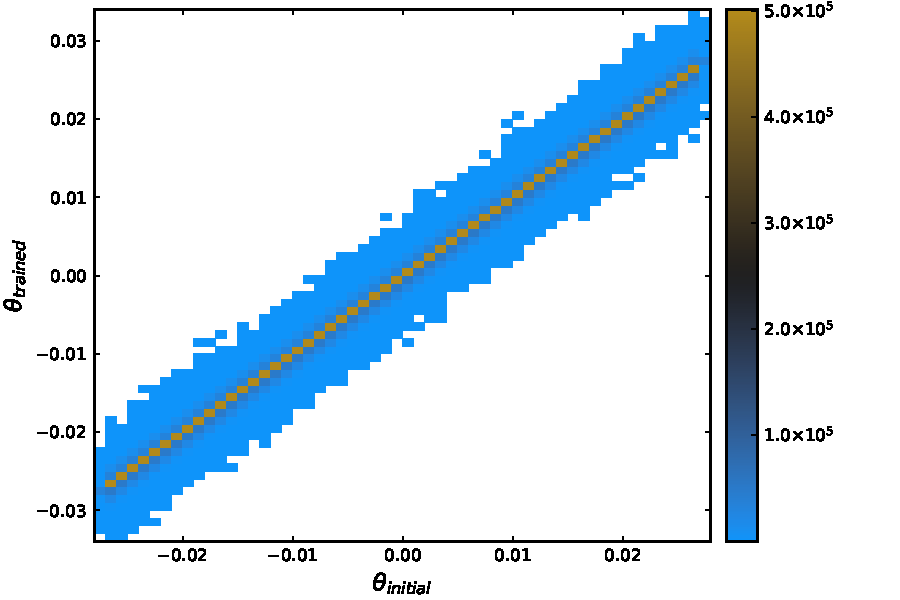
\includegraphics[width=\textwidth]{figuras/capitulo-4/weights_phi=0.35.pdf}
    \caption[Comparison between weights, $\phi=0.35$.]{Relation between the trained weights and the initial weights of $\nnet$ for $\phi=0.35$. The scale on the right-hand side represents the total number of instances for the trained-initial pair of weights.}
    \label{fig:pesos35}
\end{figure}

\subsection{Does the neural network reduce to HNC?}
For the low density regimes, HNC is an accurate approximation for the interaction potential.
Hence, the neural network is an accurate approximation. On the contrary, for high density
regimes, both approximations fail to provide an accurate solution.

If the neural network is in indeed oscillating about zero (the HNC approximation), then
it makes sense that both estimations give the results observed. Yet, we cannot guarantee
by any means possible that the neural network reduces to the HNC approximation.
We only possess \emph{statistical evidence} from the training dynamics that the neural
network weights do not change much throughout its training.

This observation might shed light into possibilities of changing the way the neural
network propagates its values and return an output. For example, a modification to the
neural network topology might be in order, such that introducing important 
nonlinearities that are consistent with the physical properties of the system can yield
better results. For the case of hard spheres, the work by Malijevský and Labík~\cite{malijevskyBridgeFunctionHard1987}
shows that the bridge function has particular functional properties, such that the
bridge function is non-negative and oscillating, among others. These properties can then
be consolidated within the neural network structure and investigate if the neural network 
weights change considerably.
From this, one might expect two outcomes. Firstly, the case where the \emph{weights change},
which would indicate that adding nonlinearities according to some aspect of the interaction 
potential prove benefitial for the weight update and training dynamics.
Secondly, the case where the \emph{weights do not change}, in which case we might
be able the have stronger evidence that, regardless of the neural network structure,
this kind of approximation will have a high chance of reproducing the HNC results.
In any case, with either outcome we do not have the information to assess if the neural
network might actually be \emph{more precise} than it is in its current form.

\begin{figure}[t]
    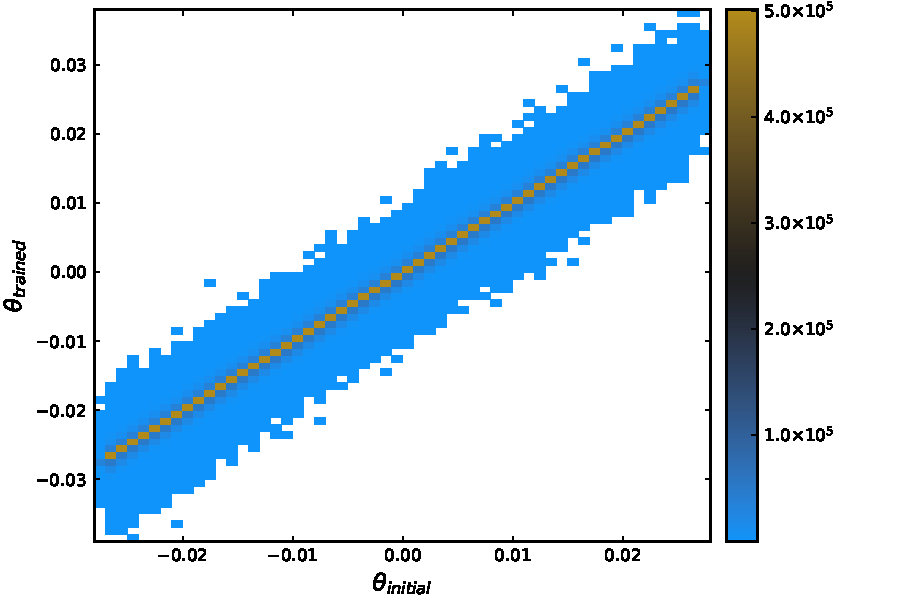
\includegraphics[width=\textwidth]{figuras/capitulo-4/weights_phi=0.45.pdf}
    \caption[Comparison between weights, $\phi=0.45$.]{Relation between the trained weights and the initial weights of $\nnet$ for $\phi=0.45$. The scale on the right-hand side represents the total number of instances for the trained-initial pair of weights.}
    \label{fig:pesos45}
\end{figure}

Similar results were found by Goodall and Lee~\cite{a.goodallDatadrivenApproximationsBridge2021}
while using data from simulations. In this approach, a data set was built with several
correlation functions that came from physical properties of the liquid. If the data set was built
just using the indirect correlation function $\gamma(\vecr)$, the neural network trained from this data
set would yield results similar or worse to those obtained with the HNC approximation.
So, in some sense, the proposed methodology here might actually be better than a fully
data-driven methodology. However, this just makes a stronger case for the argument that,
indeed, the neural network might reduce to the HNC approximation and not have enough
information about the system to adjust the weights properly.

\subsection{Neural networks as random polynomial approximations}
An interesting result from this investigation is the fact that a random approximation
provides a solution to the OZ equation. In what way is it random? Take the weights of the
neural network to be the coefficients of some \emph{random polynomial}, i.e. a polynomial 
with coefficients that come from some probability distribution $P$. This is something that 
is not trivial on why it could work as a bridge function approximation, even if the result
is very close to the HNC approximation. This would imply that, for the probability 
distribution $P$ with some finite variance $\sigma^2$ and mean $\mu=0$, the resulting
polynomial would yield a bridge function estimation similar to the HNC closure relation.
Yet, the reason why a random approximation might be a solution to the OZ equation is not
clear.

To understand the significance of this, we must recall that the bridge function can, in 
fact, be understood as a
power series in density~\cite{hansenTheorySimpleLiquids2013},
\begin{equation}
    b(\vecr) = b^{(2)}(\vecr) \rho^2 + b^{(3)}(\vecr) \rho^3 + \cdots ,
    \label{eq:expansion-densidad}
\end{equation}
where the notation $b^{(n)}(\vecr)$ indicates the $n$-particle bridge function, i.e. the
estimation of the bridge function for $n$ interacting particles. It is specially
important to note that the coefficients $b^{(n)}(\vecr)$ are, in general, high-dimensional
integrals that are mostly \emph{intractable}. Almost always, for a given bridge function
approximation, numerical methods are in order if these coefficients are to be determined.
For instance, the work by Kwak and Kofke~\cite{kwakEvaluationBridgefunctionDiagrams2005}
uses a Monte Carlo sampling numerical method to evaluate up to $b^{(4)}(\vecr)$ 
for the hard-sphere fluid. They report that even if the numerical computation is
possible, convergence is slow and computationally costly.

Only for special cases, these coefficients can be determined in closed form, e.g.
for the Percus-Yevick approximation the value of
\[
b^{(2)}(\vecr) = -\frac{1}{2}{\left[ g_{1}(\vecr) \right]}^2
\]
is known from diagrammatic methods~\cite{hansenTheorySimpleLiquids2013}. In this
expression, $g_{1}(\vecr)$ represents the single-particle radial distribution function.

Let us now understand the role of \emph{random polynomials} and their relation to the neural
network bridge function approximation used in this investigation.
Let $p_n$ be an algebraic polynomial of the form
\begin{equation}
    p_n(z) = a_0 + a_1 z + a_2 z^2 + a_3 z^3 + \cdots + a_n z^n, \quad
    z \in \mathbb{C}
    \label{eq:random-poly}
\end{equation}
where the coefficients $a_0, a_1, \dots , a_n$ are independent real-valued random variables
with finite mean and finite variance. This kind of polynomials have found successful
applications in some areas of physics~\cite{houghZerosGaussianAnalytic2009}.
These polynomials have also been the interest of mathematical research~\cite{edelmanHowManyZeros1995}.

Now, by means of the universal approximation theorem, we can regard the neural network
as a power series similar to \autoref{eq:random-poly}. To see this more clearly, we
can think of the weights of the neural network as some coefficients of a power series,
obtained under some transformation that takes in the weights and return the coefficients
needed to build a power series.
Further, if we compare directly \autoref{eq:random-poly}
and \autoref{eq:expansion-densidad}, we can see that these expressions
are related through their coefficients, with the exception of the first two terms, implying 
that random variables might be able to give an answer to the $n$ particle bridge functions 
in the power series.

Indeed, this is a convenient way of estimating the coefficients of the bridge function,
when expressed in a power series of the density or any other correlation functions.
Although, the practical way to estimate these coefficients is to enforce thermodynamic
self-consistency. Such is the case of the work by Vompe and Martynov~\cite{vompeBridgeFunctionExpansion1994},
and the work by Tsednee and Luchko~\cite{tsedneeClosureOrnsteinZernikeEquation2019}, where
the coefficients are found through a minimization problem when the thermodynamic consistency
among different routes has been achieved.

After all, the insight of random polynomials might pave the way for a novel way of 
computing coefficients by using neural networks, or related probabilistic methods.
Even though there is no way to enforce thermodynamic self-consistency when using such
methods, it is interesting to see the striking resemblance with these approaches.
And yet, one of the downsides of this is the fact that the probability
distribution for the coefficients $a_0, a_1, \dots , a_n$ cannot be known even through the
training dynamics of the neural network. A naive way of acquiring the underlying 
probability distribution is to suppose there is
a unique probability distribution and estimate its mean and variance by maximum likelihood
estimation techniques~\cite{hastieElementsStatisticalLearning2009}.
Still, even if there could be a relation between random polynomials and the bridge 
function, there can be no guarantee that the resulting approximation is good enough, or 
that it could reproduce the physics of the problem properly.
This is just mere speculation that a deeper relationship between the neural network 
approximation and the bridge function might be exploitable through the lens of random
polynomials and probability theory.

\section{Concluding remarks}
Even though neural networks can approximate any continuous function,
it is up to the implementation that uses them
to benefit from the underlying domain knowledge of the problem to be solved. In this case,
even if the methodology created is \emph{theoretically possible}, it raises the question of
whether the neural networks are the most suitable solution for the OZ equation.
Such might be the case for the methodology presented here. After all, the results
seem to \emph{strongly suggest} that a neural network reduces to one of the classic 
approximations,
the Hypernetted Chain approximation, which is not the best approximation for all kinds
of interaction potentials, and most certainly is not the case of the pseudo hard sphere
and hard sphere potentials.
At any rate, these results show a promising application of such models, in the form of
understanding how or why certain bridge function approximations provide a solution to the 
OZ equation. Unlike the use of fully data-driven methodologies, like the one from
Goodall and Lee~\cite{a.goodallDatadrivenApproximationsBridge2021},
the proposed methodology might somehow be able to provide intuition into what is happening
with the bridge function itself without the need of other theoretical methods.

One of the main drawbacks of the current proposal is the fact that the number of weights
is too large to effectively train well. This might be a reason of why the spread was
small in the weight evolution of $\nnet$. A way to alleviate this problem is to use
dimensionality reduction techniques such as
Principal Component Analysis~\cite{hastieElementsStatisticalLearning2009}. 
These methods can adequately reduce the total number of weights to be trained, without 
losing too much information from the learning dynamics.

In order to use the physics of the problem to our advantage, a different optimization
problem might be formulated, in which case a thermodynamic consistency cost function
might be able to drive the learning dynamics. In this framework, it is expected to minimize 
the difference between two different routes that compute the pressure, or the isothermal
compressibility, similar to the approaches by Zerah and Hansen~\cite{zerahSelfConsistentIntegral1986}, 
as well as Rogers and Young~\cite{rogersNewThermodynamicallyConsistent1984}.
A deficiency of such scheme is that the cost function will be
a highly nonlinear function, and possibly a \emph{black-box function}, in which case
the gradient of the function might be hard or even impossible to compute in a timely manner.
This affects not only the computation time but the ability to use gradient descent methods,
or any other optimization method that uses gradients to find an extremum.
Nevertheless, such approach could be a dramatic improvement over the methodology presented
here, even more so if coupled with a dimensionality reduction technique.

In closing, neural networks are capable models for the approximation of any continuous function, 
but domain knowledge of the problem is needed for these models to succeed when no data set 
is available. In the proposal presented in this chapter, we wanted to investigate two things, 
whether neural networks could solve the OZ equation and their quality of approximation. 
It was shown that, indeed, neural networks can solve the OZ equation, but without more 
information on the system itself, neural networks do not generalize well and their training 
dynamics suffer greatly. The bridge function approximation that these models provide is
implied to be as accurate as the Hypernetted Chain bridge function.
The information that these models gather throughout the training 
is minimal, but their training dynamics shed some light into the possibilities of using 
probability methods to approximate bridge functions in liquids.